\documentclass[12pt,aspectratio=169]{beamer}

\usetheme[
    sectionpage=progressbar,
    subsectionpage=progressbar,
    progressbar=frametitle
]{metropolis}

\definecolor{mDarkBrown}{HTML}{FF5722}
\definecolor{mDarkTeal}{HTML}{263238}
\definecolor{mLightBrown}{HTML}{FF5722}

\usepackage{booktabs}
\usepackage{graphicx}
\usepackage{hyphenat}
\usepackage{multirow}
\usepackage[normalem]{ulem}

\usepackage{pifont}
\newcommand{\cmark}{\ding{51}}
\newcommand{\xmark}{\ding{55}}

\usepackage{minted}
\usemintedstyle{tango}

\usepackage{polyglossia}
\setdefaultlanguage[variant=british]{english}
\usepackage[english=british]{csquotes}

\defaultfontfeatures{Ligatures=TeX}
\setmainfont{Lucida Sans OT}
\setsansfont[Scale=MatchLowercase]{Lucida Sans OT}
\setmonofont[Scale=MatchLowercase]{Lucida Console DK}

\author{Gianluca Campanella}
\date{}



\title{Demystifying Data Science}

\begin{document}

\maketitle

\begin{frame}{Contents}
    \tableofcontents[hideallsubsections]
\end{frame}

\section{What is Data Science?}

\begin{frame}{What is Data Science?}
    \begin{center}
        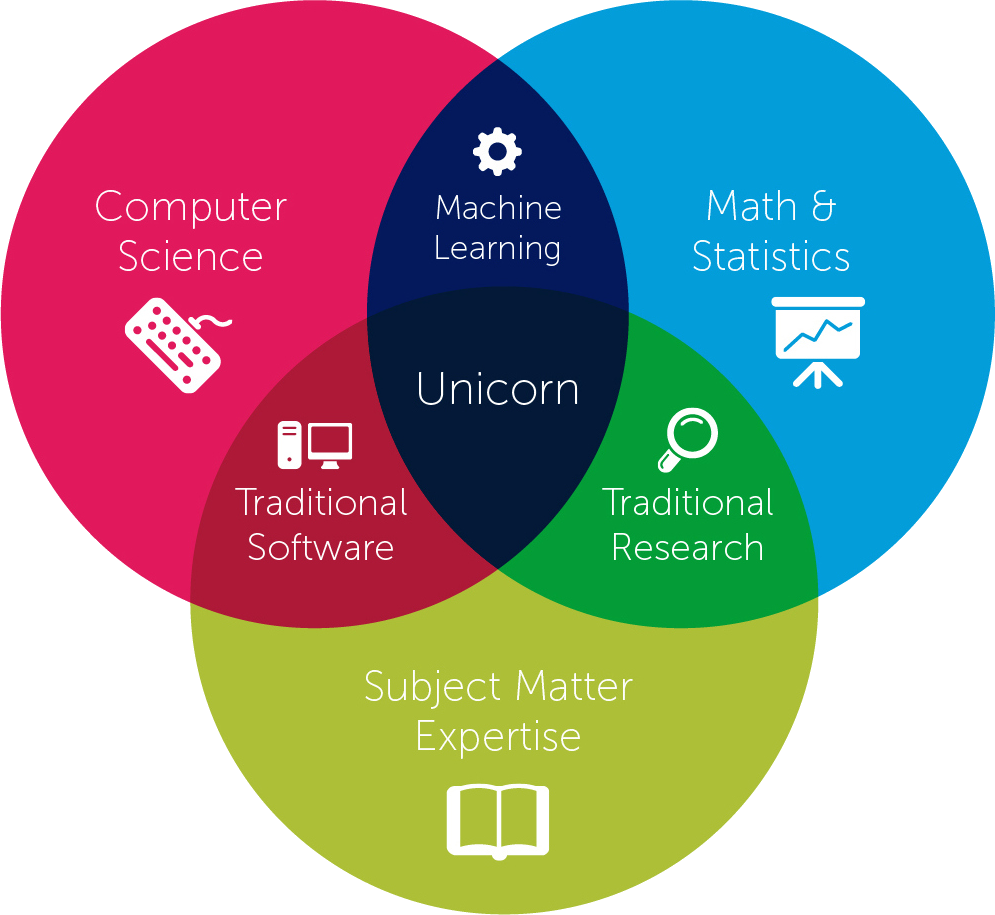
\includegraphics[height=0.8\textheight]{figures/data_science_venn_diagram} \\
        {\scriptsize%
         From S.\ Geringer (originally from D.\ Conway)}
    \end{center}
\end{frame}

\begin{frame}{How's it different from\ldots}
    \begin{itemize}
        \item Applied Mathematics?
        \item Statistics?
        \item Operational Research?
        \item Business Intelligence?
        \item Predictive Analytics?
        \item Machine Learning?
        \item Data Mining?
        \item Knowledge Discovery?
        \item Deep Learning?
        \item Artificial Intelligence?
    \end{itemize}
\end{frame}

\begin{frame}{Data Science is\ldots}
    \begin{center}
        \Large\bf%
        Data\hyp{}driven decision\hyp{}making
    \end{center}
    \vfill
    \begin{itemize}
        \item Focus is on the problem\hyp{}solving process
        \item Multidisciplinary but domain\hyp{}centric
        \item Tools are secondary!
    \end{itemize}
\end{frame}

\begin{frame}{Two types of Data Science}
    \begin{columns}
        \begin{column}{0.5\textwidth}
            \begin{center}
                \large\bf%
                Analysis\hyp{}focused
            \end{center}
            \begin{itemize}
                \item Maths and Statistics
                \item Business Intelligence
                \item[$\to$] Assist human decision\hyp{}making
            \end{itemize}
        \end{column}
        \begin{column}{0.5\textwidth}
            \begin{center}
                \large\bf%
                Building\hyp{}focused
            \end{center}
            \begin{itemize}
                \item Machine Learning
                \item Software Engineering
                \item[$\to$] Develop and deploy data\hyp{}driven products
            \end{itemize}
        \end{column}
    \end{columns}
\end{frame}

\section{What can Data Science do?}

\begin{frame}{Opportunities}
    \begin{center}
        \begin{tabular}{ll}
            \toprule
            \textbf{Domain}                      & \textbf{Applications} \\
            \midrule
            \multirow{2}{*}{Finance}             & Financial forecasting \\
                                                 & Fraud and risk management \\
            \midrule
            \multirow{2}{*}{Marketing and sales} & Churn analytics \\
                                                 & Dynamic pricing \\
            \midrule
            \multirow{3}{*}{Operations}          & Inventory optimisation \\
                                                 & Predictive maintenance \\
                                                 & Quality assurance \\
            \midrule
            \multirow{2}{*}{Workforce}           & HR analytics \\
                                                 & Resource planning \\
            \bottomrule
        \end{tabular}
    \end{center}
\end{frame}

\begin{frame}{The five questions}
    \begin{enumerate}
        \item How much/many?
        \item Is this A or B?
        \item How is this organised?
        \item Is this weird?
        \item What should I do next?
    \end{enumerate}
\end{frame}

\begin{frame}{How much/many?}
    \begin{block}{Examples}
        \begin{itemize}
            \item What will the temperature be next Sunday?
            \item What will total sales be next quarter?
        \end{itemize}
    \end{block}
    \begin{center}
        \large%
        $\downarrow$
        \vfill
        \alert{Regression} algorithms
    \end{center}
\end{frame}

\begin{frame}{Is this A or B?}
    \begin{block}{Examples}
        \begin{itemize}
            \item Which is more effective: a £10 voucher or a 10\% discount?
            \item Will this machine fail in the next month?
        \end{itemize}
    \end{block}
    \begin{center}
        \large%
        $\downarrow$
        \vfill
        \alert{Classification} algorithms
    \end{center}
\end{frame}

\begin{frame}{How is this organised?}
    \begin{block}{Examples}
        \begin{itemize}
            \item Which users like similar movies?
            \item Which items are frequently purchased together?
        \end{itemize}
    \end{block}
    \begin{center}
        \large%
        $\downarrow$
        \vfill
        \alert{Clustering} algorithms
    \end{center}
\end{frame}

\begin{frame}{Is this weird?}
    \begin{block}{Examples}
        \begin{itemize}
            \item Is this transaction fraudulent?
            \item Is this blood pressure reading normal?
        \end{itemize}
    \end{block}
    \begin{center}
        \large%
        $\downarrow$
        \vfill
        \alert{Anomaly detection} algorithms
    \end{center}
\end{frame}

\begin{frame}{What should I do next?}
    \begin{block}{Examples}
        \begin{itemize}
            \item Should the thermostat adjust the temperature?
            \item Where should the robot vacuum go next?
        \end{itemize}
    \end{block}
    \begin{center}
        \large%
        $\downarrow$
        \vfill
        \alert{Reinforcement learning} algorithms
    \end{center}
\end{frame}

\begin{frame}{Supervised vs unsupervised algorithms}
    \begin{columns}
        \begin{column}{0.5\textwidth}
            \begin{center}
                \large\bf%
                Supervised algorithms
            \end{center}
            \begin{itemize}
                \item Are trained on existing data
                \item Can be compared according to some `goodness' metric
            \end{itemize}
        \end{column}
        \begin{column}{0.5\textwidth}
            \begin{center}
                \large\bf%
                Unsupervised algorithms
            \end{center}
            \begin{itemize}
                \item Don't use examples with known outcomes
                \item Give clues, not `right answers'
            \end{itemize}
        \end{column}
    \end{columns}
\end{frame}

\begin{frame}{Data Science solutions}
    \begin{center}
        \begin{tabular}{lll}
            \toprule
            \textbf{Family}               & \textbf{Class}         & \textbf{Question} \\
            \midrule
            \multirow{2}{*}{Supervised}   & Regression             & How much/many? \\
                                          & Classification         & Is this A or B? \\
            \midrule
            \multirow{2}{*}{Unsupervised} & Clustering             & How is this organised? \\
                                          & Anomaly detection      & Is this weird? \\
            \midrule
                                          & Reinforcement learning & What should I do next? \\
            \bottomrule
        \end{tabular}
    \end{center}
\end{frame}

\section{How do you do Data Science?}

\begin{frame}{High\hyp{}level view}
    \only<1>{%
        \begin{center}
            \large%
            Business goal
            \vfill
            $\downarrow$
            \vfill
            Testable hypothesis
            \vfill
            $\downarrow$
            \vfill
            Experimentation and modelling
        \end{center}}
    \only<2>{%
        \begin{center}
            \large%
            Research question
            \vfill
            $\downarrow$
            \vfill
            Obtain $\ \longleftrightarrow\ $ Explore $\ \longleftrightarrow\ $ Model
            \vfill
            $\downarrow$
            \vfill
            Summarise / Operationalise
        \end{center}}
    \only<3>{%
        \begin{center}
            \Large%
            This process is \\
            non\hyp{}linear and iterative
        \end{center}}
\end{frame}

\begin{frame}[t]{Define the research question}
    \begin{block}{What to do}
        \begin{itemize}
            \item Identify the problem and why it should be solved
            \item Frame it in the context of data collection
        \end{itemize}
    \end{block}
    \vfill
    \begin{block}{What to ask}
        \begin{itemize}
            \item Which metrics do I need to improve?
            \item Which are possible actions to solve the problem?
            \item What is the benefit of solving the problem?
        \end{itemize}
    \end{block}
\end{frame}

\begin{frame}[t]{Obtain the data}
    \begin{block}{What to do}
        \begin{itemize}
            \item Measure the gap between ideal and available
            \item Think about assumptions and limitations
        \end{itemize}
    \end{block}
    \vfill
    \begin{block}{What to ask}
        \begin{itemize}
            \item Are there enough data?
            \item Are they relevant to the research question?
            \item Can they be trusted?
        \end{itemize}
    \end{block}
\end{frame}

\begin{frame}[t]{Explore the data}
    \begin{block}{What to do}
        \begin{itemize}
            \item Data dictionary and any other documentation
            \item Descriptive statistics and visualisations
        \end{itemize}
    \end{block}
    \vfill
    \begin{block}{What to ask}
        \begin{itemize}
            \item What kind of simple visualisations can I use?
            \item Which data types and distributions?
            \item Are there missing values or outliers?
        \end{itemize}
    \end{block}
\end{frame}

\begin{frame}[t]{Model the data}
    \begin{block}{What to do}
        \begin{itemize}
            \item Model selection and fitting
            \item Focus on inference and/or prediction
        \end{itemize}
    \end{block}
    \vfill
    \begin{block}{What to ask}
        \begin{itemize}
            \item What is an appropriate model for the data?
            \item How can I evaluate model performance?
            \item Can the model be refined?
        \end{itemize}
    \end{block}
\end{frame}

\begin{frame}[t]{Summarise the findings}
    \begin{block}{What to do}
        \begin{itemize}
            \item Storytelling and visual aids to interpretation
            \item Communicate assumptions and limitations
        \end{itemize}
    \end{block}
    \vfill
    \begin{block}{What to ask}
        \begin{itemize}
            \item How can I communicate results effectively?
            \item What format should I adopt?
            \item Who are my audience?
        \end{itemize}
    \end{block}
\end{frame}

\begin{frame}[t]{Operationalise}
    \begin{block}{What to do}
        \begin{itemize}
            \item System integration
            \item Monitoring and maintenance
        \end{itemize}
    \end{block}
    \vfill
    \begin{block}{What to ask}
        \begin{itemize}
            \item What (visual) outputs do I care about?
            \item How often does the model need retraining?
            \item Do we need to think about scalability?
        \end{itemize}
    \end{block}
\end{frame}

\section{How do you implement it?}

\begin{frame}{The secret is in the ingredients}
    Good Data Science requires:
    \begin{itemize}
        \item Tidy data
        \item Sharp questions
        \item A capable process
        \item Good people
    \end{itemize}
\end{frame}

\subsection{Tidy data}

\begin{frame}{Good data}
    \Large%
    \begin{center}
        Data Scientists
        \hspace{1em}
        \begin{tabular}{cl}
            \textbf{C} & onnected \\[0.25em]
            \textbf{A} & ccurate \\[0.25em]
            \textbf{R} & elevant \\[0.25em]
            \textbf{E} & nough \\
        \end{tabular}
        \hspace{1em}
        about data!
    \end{center}
\end{frame}

\begin{frame}{No data is better than bad data}
    \begin{center}
        {\Large%
         Bad data \,<\, no data \,<\, good data \,<\, tidy data}
    \end{center}
    \vfill
    \begin{columns}
        \begin{column}{0.5\textwidth}
            \begin{block}{Bad data}
                \begin{itemize}
                    \item Duplicate
                    \item Missing
                    \item Inaccurate or incorrect
                \end{itemize}
            \end{block}
        \end{column}
        \begin{column}{0.5\textwidth}
            \begin{block}{Tidy data}
                \begin{itemize}
                    \item Variables $\to$ columns
                    \item Observation $\to$ rows
                    \item Types $\to$ tables
                \end{itemize}
            \end{block}
        \end{column}
    \end{columns}
\end{frame}

\begin{frame}{How much data do I need?}
    \begin{itemize}
        \item Appropriateness is normally more important
        \item However, there are certain statistical requirements\ldots
    \end{itemize}
    \begin{center}
        \begin{tabular}{lr}
            \toprule
            \textbf{Type of analysis} & \multicolumn{1}{l}{\textbf{Sample size}} \\
            \midrule
            Summary statistics & > 10      \\
            Parametric models  & > 100     \\
            Most ML models     & > 1,000   \\
            Deep Learning      & > 100,000 \\
            \bottomrule
        \end{tabular}
    \end{center}
\end{frame}

\begin{frame}{Don't try to run before you can walk}
    \begin{center}
        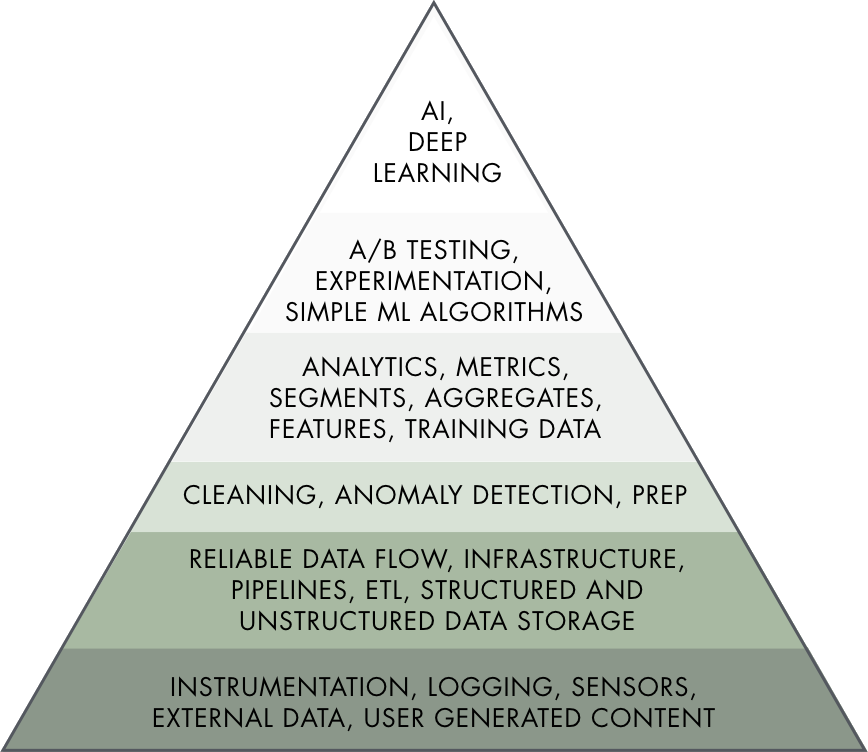
\includegraphics[height=0.8\textheight]{figures/ai_hierarchy} \\
        {\scriptsize%
         From M.\ Rogati}
    \end{center}
\end{frame}

\subsection{Sharp questions}

\begin{frame}{Sharp questions}
    \only<1>{%
        \large%
        \begin{quote}
            What people think of as the moment of discovery is really the
            discovery of the question.

            \begin{flushright}
                --- J.\ E.\ Salk
            \end{flushright}
        \end{quote}}
    \only<2>{%
        \begin{center}
            \Large%
            Sharp questions can be answered with data
        \end{center}
        \begin{itemize}
            \item[$\rightarrow$] Give clues as to which algorithms can answer them
            \item[$\rightarrow$] Help identify the target data
            \item[$\rightarrow$] Can be rephrased to give more useful answers
        \end{itemize}
        \vfill
        \begin{itemize}
            \item[\xmark] What's going to happen with sales?
            \item[\cmark] What will total sales be next quarter?
        \end{itemize}}
\end{frame}

\begin{frame}{Modelling misconceptions}
    Most well\hyp{}executed data science projects don't\ldots
    \begin{itemize}
        \item Use complicated tools
        \item Fit complicated models
    \end{itemize}
    \vfill
    Instead, they do\ldots
    \begin{itemize}
        \item Focus on solving the problem
        \item Use appropriate --- not necessarily big! --- data
        \item Use relatively standard models
    \end{itemize}
\end{frame}

\begin{frame}{The 80---20 rule of modelling}
    \begin{itemize}
        \item The first reasonable thing you can do goes 80\% of the way
        \item Everything after that is to get the remaining 20\%\ldots \\
              often at additional cost!
    \end{itemize}
    \vfill\pause
    \begin{center}
        \Large%
        Is it worth it?
    \end{center}
\end{frame}

\begin{frame}{Know your domain}
    Domain knowledge allows you to\ldots
    \begin{itemize}
        \item Understand possible data collection flaws
        \item Identify feature dependence and leakage
        \item Create new features (feature engineering)
        \item Interpret your results correctly
        \item Be understood by stakeholders
    \end{itemize}
\end{frame}

\subsection{A capable process}

\begin{frame}{A Data Scientist's dream}
    In an ideal world there are\ldots
    \begin{itemize}
        \setlength{\itemsep}{0.75em}
        \item Tidy data
        \item Sharp questions
        \item Resources and time to experiment and model
    \end{itemize}
\end{frame}

{
    \usebackgroundtemplate{%
        
\includegraphics[width=\paperwidth,height=\paperheight]{figures/frustration}}
    \begin{frame}{The sad reality\ldots}
    \end{frame}
}

\begin{frame}{What's a capable process?}
    \begin{center}
        \large%
        Are you maximising\ldots
    \end{center}
    \begin{columns}
        \begin{column}{0.5\textwidth}
            \begin{center}
                {\large\bf%
                 Certainty} \\[1em]
                `Unchanging' truths \\[1em]
                $\downarrow$ \\[1em]
                {\large%
                 Science}
            \end{center}
        \end{column}
        \begin{column}{0.5\textwidth}
            \begin{center}
                {\large\bf%
                 Growth rate} \\[1em]
                Changing truths \\[1em]
                $\downarrow$ \\[1em]
                {\large%
                 Adversarial industries}
            \end{center}
        \end{column}
    \end{columns}
\end{frame}

\begin{frame}{ROI of Data Science projects}
    \begin{center}
        \large%
        No one knows which projects will have the best ROI!
    \end{center}
    \vfill
    \begin{itemize}
        \item Power law\hyp{}like distribution of returns
        \item[$\rightarrow$] Do several projects in short sprints
    \end{itemize}
    \begin{itemize}
        \item Failure is always an option!
        \item[$\rightarrow$] Learn when to cut losses
    \end{itemize}
\end{frame}

\begin{frame}{Agile Data Science}
    \begin{center}
        \Large%
        {\bf%
         High\hyp{}risk, high\hyp{}reward innovation culture}
        \vfill
        \begin{tabular}{rcl}
        \multirow{3}{*}{\textbf{Data strategy}} &       & Product roadmap \\
                                                & $\to$ & Data collection \\
                                                &       & Leadership buy\hyp{}in \\
        \end{tabular}
    \end{center}
\end{frame}

\subsection{Good people}

\begin{frame}{Good people}
    \begin{itemize}
        \item Traditional analysts often focused on specific tools
        \item Many programmers don't have business experience
    \end{itemize}
    \vfill\pause
    Successful Data Scientists are\ldots
    \begin{itemize}
        \item Practical, impact\hyp{}driven, dependable people
        \item Passionate about their domain
        \item Knowledgeable about research methods and statistics
        \item Coding ninjas
    \end{itemize}
\end{frame}

\begin{frame}{Good teams}
    Successful Data Science teams are\ldots
    \begin{itemize}
        \item Flexible and open
        \item Diverse
        \item Collaborative
    \end{itemize}
\end{frame}

\end{document}

